\graphicspath{{./chapters/chapter2/}}
%\newtheorem{thm}{Theorem}
%\newtheorem{lem}[thm]{Lemma}
%\DeclareMathOperator*{\argmax}{arg\,max}
%\DeclareMathOperator*{\argmin}{arg\,min}

\def\D{{\mathcal D}}
\def\Pphi{\overline{\Phi}}
\def\F{{\mathcal F}}
\def\N{{\mathcal N}}
%\def\R{{\mathbb R}}
\def\E{{\mathbb E}}
\def\A{\Pi}
\def\B{\Sigma}
\def\diam{\text{diam}}
\def\c{\mathcal L}
\def\l{\ell}
\def\seq{seq}
\def\R{\mathbb{R}}
\def\C{\mathcal C}
\def\p{p}
\def\s{size}
\def\L{\mathcal L}
\def\o{opt}
\def\H{\mathcal H}
\def\calH{\mathcal H}
\def\of{approxCluster}
\def\on{onlineCluster}
\def\R{\mathbb R}
\def\Y{\{\pm 1\}}
\def\U{\mathbb U}
\def\dd{\Delta}
\def\simp{{U\Delta}}
\def\g{g}
\def\rr{R}
\def\f{f}


\chapter{Sample Complexity of Robust Linear Classification on Separated Data} 

\section{Introduction}

Motivated by the use of machine learning in safety-critical settings, adversarially robust classification has been of much recent interest. Formally, the problem is as follows. A learner is given training data drawn from an underlying distribution $D$, a hypothesis class $\calH$, a robustness metric $d$, and a radius $r$. The learner's goal is to find a classifier $h \in \calH$ which has the lowest robust loss at radius $r$. The robust loss of a classifier is the expected fraction of examples where either $f(x) \neq y$ or where there exists an $x'$ at distance $d(x, x') \leq r$ such that $f(x) \neq f(x')$.  Robust classification thus aims to find a classifier that maximizes accuracy on examples that are distance $r$ or more from the decision boundary, where distances are measured according to the metric $d$.


In this work, we ask: how many samples are needed to learn a classifier with low robust loss when $\calH$ is the class of linear classifiers, and $d$ is an $\ell_p$-metric? Prior work has provided both upper~\cite{bartlett19, ravikumar20} as well as lower bounds~\cite{Schmidt18, ravikumar20} on the sample complexity of the problem. However, almost all look at settings where the data distribution itself is not separated --  data from different classes overlap or are close together in space. In this case, the classifier that minimizes robust loss is quite different from the one that minimizes error, which often leads to strong sample complexity gaps. Many real tasks where robust solutions are desired however tend to involve well-separated data~\cite{Yang20}, and hence it is instructive to look at what happens in these cases.

With this motivation, we consider in this work robust classification of data that is linearly $r$-separable. Specifically, there exists a linear classifier which has zero robust loss at robustness radius $r$. This case is thus the analog of the realizable case for robust classification, and we consider both upper and lower bounds in this setting.

For lower bounds, prior work \cite{Cullina18} shows that both standard and robust linear classification have VC-dimension $O(d)$, and consequently have similar bounds on the expected loss in the worst case. However, these results do not apply to this setting since we are specifically considering well-separated data, which greatly restricts the set of possible worst-case distributions.  For our lower bound, we provide a family of distributions that are linearly $r$-separable and where the maximum margin classifier, given $n$ independent samples, has error $O(1/n)$. In contrast, any algorithm for finding the minimum robust loss classifier has robust loss at least $\Omega(d/n)$, where $d$ is the data dimension. These bounds hold for all $\ell_p$-norms provided $p > 1$, including $p=2$ and $p=\infty$. Unlike prior work, our bounds do not rely on the difference in loss between the solutions with optimal robust loss and error, and hence cannot be obtained by prior techniques. Instead, we introduce a new geometric construction that exploits the fact that learning a classifier with low robust loss when data is linearly $r$-separated requires seeing a certain number of samples close to the margin.

For upper bounds, prior work \cite{bartlett19} provides a bound on the Rademacher complexity of adversarially robust learning, and show that it can be worse than the standard Rademacher complexity by a factor of $d^{1/q}$ for $\ell_p$-norm robustness where $1/p + 1/q = 1$. Thus, an interesting question is whether dimension-independent bounds, such as those for the accuracy under large margin classification, can be obtained for robust classification as well. Perhaps surprisingly, we show that when data is really well-separated, the answer is yes. Specifically, if the data distribution is linearly $r + \gamma$-separable, then there exists an algorithm that will find a classifier with robust loss $O(\Delta^2/\gamma^2 n)$ at radius $r$ where $\Delta$ is the diameter of the instance space. Observe that much like the usual sample complexity results on SVM and perceptron, this upper bound is independent of the data dimension and depends only on the excess margin (over $r$). This establishes that when data is really well-separated, finding robust linear classifiers does not require a very large number of samples. 

While the main focus of this work is on linear classifiers, we also show how to generalize our upper bounds to Kernel Classification, where we find a similar dynamic with the loss being governed by the excess margin in the embedded kernel space. However, we defer a thorough investigation of robust kernel classification as an avenue for future work.

Our results imply that while adversarially robust classification may be more challenging than simply accurate classification when the classes overlap, the story is different when data is well-separated. Specifically, when data is linearly (exactly) $r$-separable, finding an $r$-separated solution to robust loss $\epsilon$ may require $\Omega(d/\epsilon)$ samples for some distribution families where finding an accurate solution is easier. Thus in this case, there is a gap between the sample complexities of robust and simply accurate solutions, and this is true regardless of the $\ell_p$ norm in which robustness is measured. In contrast, if data is even more separated -- linearly $r + \gamma$-separable --  then we can obtain a dimension-independent upper bound on the sample complexity, much like the sample complexity of SVMs and perceptron. Thus, how separable the data is matters for adversarially robust classification, and future works in the area should consider separability while discussing the sample complexity.

\subsection{Related Work}

There is a large body of work \cite{Carlini17, Liu17, Papernot17, Papernot16, Szegedy14, Hein17, Katz17, Wu16,Steinhardt18, Sinha18} empirically studying adversarial examples primarily in the context of neural networks. Several works \cite{Schmidt18, Raghunathan20, Tsipras19} have empirically investigated trade-offs between robust and standard classification.

On the theoretical side, this phenomenon has been studied in both the parametric and non-parametric settings. On the parametric side, several works \cite{loh18, attias19, Srebro19, bartlett19, pathak20} have focused on finding distribution agnostic bounds of the sample complexity for robust classification. In \cite{Srebro19}, Srebro et. al. showed through an example that the VC dimension of robust learning may be much larger than standard or accurate learning indicating that the sample complexity bounds may be higher. However, their example did not apply to linear classifiers. 

\cite{Kane20} considers learning linear classifiers robustly, but is primarily focused on computational complexity as opposed to sample complexity.

In \cite{bartlett19}, Bartlett et. al. investigated the Rademacher complexity of robustly learning linear classifiers as well as neural networks. They showed that in both cases, the robust Rademacher complexity can be bounded in terms of the dimension of the input space -- thus indicating a possible gap between standard and robust learning. However, as with the works considering VC dimension, this work is fundamentally focused on upper bounds  -- they do not show true lower bounds on data requirements.

Because of it's simplicity and elegance, the case where the data distribution is a mixture of Gaussians has been particularly well-studied. The first such work was \cite{Schmidt18}, in which Schmidt et. al. showed an $\Omega(\sqrt{d})$ gap between the standard and robust sample complexity for a mixture of two Gaussians using the $\ell_\infty$ norm. This was subsequently expanded upon in \cite{Bhagoji19}, \cite{robey20} and  \cite{ravikumar20}. \cite{Bhagoji19} introduces a notion of ``optimal transport," which they subsequently apply to the Gaussian case, deriving a closed form expression for the optimally robust linear classifier. Their results apply to any $\ell_p$ norm. \cite{robey20} applies expands upon \cite{Schmidt18} by consider mixtures of three Gaussians in both the $\ell_2$ and $\ell_\infty$ norms. Finally, \cite{ravikumar20} fully generalizes the results of \cite{Schmidt18} providing tight upper and lower bounds on the standard and robust sample complexities of a mixture of two Gaussians, in any norm (including $\ell_p$ for $p \in [1, \infty]$). \cite{Schmidt18} and \cite{ravikumar20} bear the most relevance with our work, and we consequently carefully compare our results in section \ref{sec:comparison}.

Another approach for lower and upper bounds on sample complexities for linear classifiers can be found in \cite{Cullina18}, which examines the robust VC dimension of learning linear classifiers. They show that the VC dimension is $d+1$, just as it is in the standard case. This implies that the bounds in the robust case match the bounds in the standard case and in particular shows a lower bound of $\Omega(d/n)$ on the expected loss of learning a robust linear classifier from $n$ samples.

While this result appears to match our lower bound, there is a crucial distinction between the bounds. Our bound implies that there exists some distribution with a large $\ell_2$ margin for which the expected robust loss must be $\Omega(d/n)$. On the other hand, standard results about learning linear classifiers on large margin data implies that the expected standard loss will be $O(1/n)$ (when running the max-margin algorithm). For this reason, our paper provides a case in the well-separated setting in which learning linear classifiers is provably more difficult (in terms of sample complexity) in the robust setting than in the standard setting. By contrast, \cite{Cullina18} does not show this. Their paper only implies (through standard VC constructions) the existence of \textit{some} distribution that is difficult to learn, and the standard PAC bounds cannot ensure that such a distribution also has a large $\ell_2$ margin.

In the non-parametric setting, there are several works which contrast standard learning with robust learning. \cite{WJC18} considers the nearest neighbors algorithm, and shows how to adapt it for converging towards a robust classifier. In \cite{YRWC19}, Yang et. al. propose the $r$\textit{-optimal classifier}, which is the robust analog of the Bayes optimal classifier. Through several examples they show that it is often a fundamentally different classifier - which can lead to different convergence behavior in the standard and robust settings. \cite{Bhattacharjee20} unified these approaches by specifying conditions under which non-parametric algorithms can be adapted to converge towards the $r$-optimal classifier, thus introducing $r$-consistency, the robust analog of consistency.

\section{Preliminaries}
We consider binary classification over $\R^d \times \Y$. Our metric of choice is the $\ell_p$ norm, where $p > 1$ (including $p = \infty$) is arbitrary. For $x \in \R^d$, we will use $||x||_p$ to denote the $\ell_p$ norm of $x$, and consequently will use $||x - y ||_p$ to denote the $\ell_p$ distance between $x$ and $y$. We will also let $\ell_q$ denote the dual norm to $\ell_p$ - that is, $\frac{1}{q} + \frac{1}{p}= 1$.

 We use $B_p(x,r)$ to denote the closed $\ell_p$ ball with center $x$ and radius $r$. For any $S \subset \R^d$, we let $diam_p(S)$ denote its diameter: that is, $diam_p(S) = \sup_{x, y \in S} ||x - y||_p.$

\subsection{Standard and Robust Loss}

In classical statistical learning, the goal is to learn an accurate classifier, which is defined as follows:

\begin{defn}
Let $\D$ be a distribution over $\R^d \times \Y$, and let $f \in \Y^{\R^d}$ be a classifier. Then the \textbf{standard loss} of $f$ over $\D$, denoted $\L(f, \D)$, is the fraction of examples $(x,y) \sim \D$ for which $f$ is not accurate. Thus $$\L(f, \D) = P_{(x,y) \sim \D}[f(x) \neq y].$$
\end{defn}

Next, we define robustness, and the corresponding robust loss.

\begin{defn}
A classifier $f \in \Y^{\R^d}$ is said to be \textbf{robust} at $x$ with radius $r$ if $f(x) = f(x')$ for all $x' \in B_p(x,r)$. 
\end{defn}


\begin{defn}
The \textbf{robust loss} of $f$ over $\D$, denoted $\L_r(f, \D)$, is the fraction of examples $(x,y) \sim \D$ for which $f$ is either inaccurate at $(x,y)$, or $f$ is not robust at $(x,y)$ with radius $r$. Observe that this occurs if and only if there is some $x' \in B_p(x,r)$ such that $f(x') \neq y$. Thus $$\L_r(f, \D) = P_{(x, y) \sim \D}[\exists x' \in B_p(x,r)\text{ s.t. }f(x') \neq y].$$ 
\end{defn}

\subsection{Expected Loss and  Sample Complexity}

The most common way to characterize the performance of a learning algorithm is through an $(\epsilon, \delta)$ guarantee, which computes $\epsilon_n, \delta_n$ such that an algorithm trained over $n$ samples has loss at most $\epsilon_n$ with probability at least $1 - \delta_n$. 

In this work, we use the simpler notion of \textit{expected loss}, which is defined as follows: 

\begin{defn}
Let $A$ be a learning algorithm and let $\D$ be a distribution over $\R^d \times \{\pm 1\}$. For any $S \sim \D^n$, we let $A_S$ denote the classifier learned by $A$ from training data $S$. Then the \textbf{expected standard loss} of $A$ with respect to $\D$, denoted $EL^n(A, \D)$ where $n$ is the number of training samples, is defined as $$E\L^n(A, \D) = \E_{S \sim \D^n} \L(A_S, \D).$$ Similarly, we define the \textbf{expected robust loss} of $A$ with respect to $\D$ as $$E\L_r^n(A , \D) = \E_{S \sim \D^n}\L_r(A_S, \D).$$ 
\end{defn}

Our main motivation for using this criteria is simplicity. Our primary goal is to compare and contrast the performances of algorithms in the standard and robust cases, and this contrast clearest when the performances are summarized as a single number (namely the expected loss) rather than an $(\epsilon, \delta)$ pair. 

Next, we address the notion of sample complexity. As above, sample complexity is typically defined as the minimum number of samples needed to guarantee $(\epsilon, \delta)$ performance. In this work, we will instead define it solely with respect to $\epsilon$, the expected loss. 

\begin{defn}
Let $\D$ be a distribution over $\R^d \times \{\pm 1\}$ and $A$ be a learning algorithm. Then the \textbf{standard sample complexity} of $A$ with respect to $\D$, denoted $m^\epsilon(A, \D)$, is the minimum number of training samples needed such that $A$ has  expected standard loss at most $\epsilon$. Formally, $$m^\epsilon(A, \D) = \min(\{n: E\L^n(A, D) \leq \epsilon\}).$$ Similarly, we can define the \textbf{robust sample complexity} as $$m_r^\epsilon(A, \D) = \min(\{n: E\L^n(A, D) \leq \epsilon\}).$$
\end{defn}

\subsection{Linear classifiers}

In this work, we consider linear classifiers, formally defined as follows:
\begin{defn}
Let $w \in \R^d$ be a vector. Then the \textbf{linear classifier} with parameters $w \in \R^d$ and $b \in \R$ over $\R^d \times {\pm 1}$, denoted $f_{w, b}$, is defined as , $$f_{w,b}(x) = \begin{cases} +1 & \langle w, x \rangle  \geq b \\ -1 & \langle w, x \rangle < b  \end{cases}.$$ 
\end{defn}

Learning linear classifiers is well understood in the standard classification setting. We now consider the linearly \textit{separable} case, in which some linear classifier has perfect accuracy. We will later define linear $r$-separability as the robust analog of separability.

\begin{defn}
A distribution $\D$ over $\R^d \times Y$ is \textbf{linearly separable} if its support can be partitioned into sets $S^+$ and $S^-$ such that:

1. $S^+$ and $S^-$ correspond to the positively and negatively labeled subsets of $\R^d$. In particular, $P_{(x,y) \sim \D}[x \in S^y] = 1.$

2. There exists a linear classifier, $f_{w, b}$, that has perfect accuracy. That is, $\L(f_{w, b}, \D) = 0$. 
\end{defn}

The standard sample complexity for linearly separable distributions can be characterized through their margin, which is defined as follows.

\begin{defn}\label{defn:margin}
Let $\D$ be a linearly separable distribution over $\R^d \times \{\pm 1\}$. Let $S^+$ and $S^-$ be as above. Then $\D$ has \textbf{margin} $\gamma$ if $\gamma$ is the largest real number such that there exists a linear classifier $f_{w,b}$ with the following properties:

1. $f_{w,b}$ has perfect accuracy. That is, $\L(f_{w,b}, \D) = 0$.

2. Let $H_{w,b} = \{x: \langle x, w \rangle = b\}$ denote the decision boundary of $f_{w,b}$. Then for all $x \in (S^+ \cup S^-)$, $x$ has $\ell_2$ distance at least $\gamma$ from $H_{w,b}$. That is, $$\inf_{x \in S^+ \cup S^-, z \in H_{w,b}} ||x - z||_2 \geq \gamma.$$ We let $\gamma(\D)$ denote the margin of $\D$.
\end{defn}

Observe that although we use a general norm, $\ell_p$, to measure robustness, the margin is always measured in $\ell_2$. This is because the $\ell_2$ norm plays a fundamental role in  bounding the number of samples needed to learn a linear classifier. 

The basic idea is that when the $\ell_2$ margin is large relative to the $\ell_2$ diameter of the distribution, the max margin algorithm requires fewer samples needed to learn a linear classifier. In particular, the ratio between the $\ell_2$ margin and the $\ell_2$ diameter fully characterizes the standard sample complexity of the max margin algorithm. To further simplify our notation, we define this ratio as the aspect ratio.

\begin{defn}\label{defn:aspect_ratio}
Let $\D$ be a linearly separable distribution over $\R^d \times \{\pm 1\}$. Then the \textbf{aspect ratio} of $\D$, $\rho(\D)$ is defined as, $$\rho(\D) = \frac{diam_2(S^+ \cup S^-)}{\gamma(\D)},$$ where $\diam_2(S^+ \cup S^-)$ denotes its diameter in the $\ell_2$ norm.
\end{defn}

We now have the following well-known result, which characterizes the expected standard loss with the aspect ratio.
\begin{thm}\label{thm:standard}
\emph{(Chapter 10 in \cite{vapnik1998})} Let $M$ denote the hard margin SVM algorithm. If $\D$ is a distribution with aspect ratio $\rho = \rho(\D)$, then for any $n > 0$ we have $\E_{S \sim \D^n}\L(M_S, \D) \leq O(\frac{\rho^2}{n}),$ where $M_S$ denotes the classifier learned by $M$ from training data $S$. 
\end{thm}

We can also express this result in terms of standard sample complexity.
\begin{cor}\label{cor:standard}
Let $M$ denote the hard margin SVM algorithm. If $\D$ is a distribution with aspect ratio $\rho = \rho(\D)$, then for any $\epsilon > 0$ we have $m^\epsilon(M_S, \D) \leq O(\frac{\rho^2}{\epsilon}),$ where $M_S$ denotes the classifier learned by $M$ from training data $S$. 
\end{cor}

Theorem \ref{thm:standard} and Corollary \ref{cor:standard} will serve as a benchmark for comparison with the robust sample complexity.  
\subsection{Linear $r$-separability}

Finally, we introduce linear $r$-separability, which is the key characteristic of distributions considered in this paper. This can be thought of as the robust analog of linear separability.
\begin{defn}\label{defn:r_separability}
For any $r > 0$, a distribution $\D$ over $\R^d \times \{\pm 1\}$ is \textbf{linearly} $r$-\textbf{separable} if there exists a linear classifier $f_{w, b}$ such that $\L_r(f_{w, b}, \D) = 0$.
\end{defn}
This definition is the fundamental property considered in this paper. Our goal is to understand the sample complexity required for learning robust linear classifiers on linearly $r$-separable distributions, and compare it with the standard sample complexity given in Theorem \ref{thm:standard}.

\section{Lower Bounds}\label{sec:lower_bounds}

In this section, we consider $r$-separated distributions whose aspect ratio is constant. By Theorem \ref{thm:standard}, the standard sample complexity for learning them is independent of $d$. We will show that in contrast, the robust sample complexity has a linear dependence on $d$, and consequently establish a substantial gap between the standard and robust cases.

We begin by defining the family of such distributions.
\begin{defn}
For any $\rho, r$, the set $\F_{r, \rho}$ is defined as the set of all distributions $\D$ over $\R^d \times \{\pm 1\}$ such that $\D$ is $r$-separated and has aspect ratio at most $\rho$.
\end{defn} 

We now state our main result.
\begin{thm}\label{thm:lower}
Let $r > 0$ and $\rho > 20$. Then the following hold.
\begin{enumerate}
	\item For every learning algorithm $A$, and any $n > 0$, there exists $\D \in \F_{r, \rho}$ such that the expected robust loss when $A$ is trained on a sample of size $n$ from $\D$ is at least $\Omega(\frac{d}{n})$. Formally, there exists a constant $c > 0$ such that $\E_{S \sim \D^n}[\L_r(A_S, \D)] \geq \frac{cd}{n}.$
	\item  In contrast, by Theorem \ref{thm:standard}, for \textit{any} $\D \in \F_{r, D}$, the max margin algorithm has expected standard loss $O(\frac{\rho^2}{n})$, when trained on a sample of size $n$ from $\D$. Formally, there exists a constant $c' > 0$ such that $\E_{S \sim \D^n}[\L(A_S, \D)] \leq \frac{c'\rho^2}{n}.$
\end{enumerate}
\end{thm}
The condition $\rho > 20$ is required to rule out degenerate cases. This is because for small values of $\rho$, the $\ell_2$ diameter of $\D$ is not much larger than the $\ell_2$ margin of $\D$. This forces $\D$ to be mostly clustered around a line which leads to more complicated behavior.

Observe that when $\rho$ is a constant independent of $d$, the expected  standard loss is $O(\frac{1}{n})$ while the expected robust loss is $\Omega(\frac{d}{n})$. Thus, the ratio between the expected robust loss and the expected standard loss is $\Omega(d)$, leading to a dimensional dependent gap between the robust and standard cases. 

We also note that these bounds hold regardless of which $\ell_p$ ($p \in (1, \infty])$ norm is being used. This is because our construction of $\D \in \F_{r, \rho}$ for which the lower bound holds is given in terms of the norm $p$. More generally, the family $\F_{r, \rho}$ is implicitly defined with respect to $p$.

Furthermore, our lower bound differs from the lower bound of $\Omega(\frac{d}{n})$ shown in prior work \cite{Cullina18} because it specifically holds for $\F_{r, \rho}$, a linearly $r$-separated family of distributions with constant aspect ratio. Thus, while \cite{Cullina18} has shown the existence of distributions satisfying the first condition of Theorem \ref{thm:lower}, our result is the first to exhibit a distribution satisfying both conditions.


Finally, we note that Theorem \ref{thm:lower} can also be expressed in terms of sample complexities. We include this in the following corollary.

\begin{cor}
Let $r > 0$ and $\rho > 20$. Then the following hold.

1. For every learning algorithm $A$, and any $\epsilon > 0$, there exists $\D \in \F_{r, \rho}$ such that the robust sample complexity of $A$ with respect to $\D$ is at least $\Omega(\frac{d}{\epsilon})$. Formally, there exists a constant $c > 0$ such that $m_r^\epsilon(A, \D) \geq \frac{cd}{\epsilon}.$

2. In contrast, by Theorem \ref{thm:standard}, for \textit{any} $\D \in \F_{r, D}$, the max margin algorithm has standard sample complexity $O(\frac{\rho^2}{\epsilon})$. Formally, there exists a constant $c' > 0$ such that $m^\epsilon(A, \D) \leq \frac{c'\rho^2}{\epsilon}.$

\end{cor}

\subsection{Comparison with \cite{ravikumar20} and~\cite{Schmidt18}}\label{sec:comparison}

The first work to provide a robust sample complexity lower bound that applied to linear classifiers is~\cite{Schmidt18}; they showed a gap of $\Omega(\sqrt{d})$ between the robust and accuracy loss for a specific mixture of two Gaussians. This was later generalized to mixtures of any two Gaussians by~\cite{ravikumar20}, who also established more general lower bounds for any $\ell_p$ norm. Since \cite{ravikumar20} is a strict generalization of \cite{Schmidt18}, we next explain how our lower bounds differ from~\cite{ravikumar20}, and why their techniques do not lead to our results. We begin by summarizing their results.

\paragraph{Summary of \cite{ravikumar20}} \cite{ravikumar20} considers data distributions $\D$ that are parametrized by $\mu \in \R^d$ and $\Sigma \in \R^{d \times d}$, $\Sigma \succcurlyeq 0$. $\D_{\mu, \Sigma}$ is the mixture of two Gaussians, $\N(\mu, \Sigma)$ and $\N(-\mu, \Sigma)$, with equal mass, where instances drawn from $\N(\mu, \Sigma)$ are labeled as $+$, and instances drawn from $\N(-\mu, \Sigma)$ are labeled as $-$. They consider robustness measured in any normed metric in $\R^d$, including the $\ell_p$ norm for $p \in (1, \infty]$. Although their bounds apply to any classifier, this effectively deals with linear classifiers since it can be shown that the optimally robust and accurate classifiers are both linear.

For any distribution $\D_{\mu, \Sigma}$, let $L_{rob}$ denote the optimal robust loss of any classifier on $\D_{\mu,\Sigma}$, and let $L_{std}$ denote the optimal standard loss. Then the bounds shown in \cite{ravikumar20} can restated as follows (a detailed derivation from \cite{ravikumar20} appears in Appendix \ref{sec:appendix_comparison}). 

\begin{thm}\label{thm:ravikumar}
\cite{ravikumar20}
\begin{enumerate}
	\item For any learning algorithm $A$ and any $n > 0$, there exists some mixture of Gaussians, $\D_{\mu, \Sigma}$ such that the expected \textit{excess} robust loss is at least $\Omega(L_{rob}\frac{d}{n}),$ when $A$ is trained on a sample of size $n$ from $\D$. 
	\item For any distribution $\D_{\mu, \Sigma}$, it is possible to learn a classifier with expected \textit{excess} standard loss at most $O(L_{std}\frac{d}{n})$.
	\item By (1.) and (2.), the ratio between the expected excess loss and expected excess standard loss can be expressed as $ratio \geq \Omega(\frac{L_{rob}}{L_{std}}).$
\end{enumerate}
\end{thm}

Observe that their bounds are given through \textit{excess} losses, which is the amount by which the loss exceeds to the optimal loss. This is necessary because in their setting, the optimal classifiers do not have $0$ loss. 

\paragraph{Comparison with our bounds} Recall that in our work, we are concerned with the \textit{linearly $r$-separated case}, which occurs precisely when the optimal robust and standard losses both equal $0$. However, from Theorem \ref{thm:ravikumar}, we see that although \cite{ravikumar20} proves a gap between standard and robust sample complexity, this gap is predicated on distributions for which the optimal robust loss, $L_{rob}$ and optimal standard loss, $L_{std}$ differ. Furthermore, in the case where they obtain a gap of $\Omega(d)$, we see that this requires $\frac{L_{rob}}{L_{std}} = \Omega(d)$ which is a substantial difference. By contrast, our results characterize a gap exclusively in the case that this does not occur. 

Finally, in the limiting case where the Gaussians they consider are sufficiently far apart, their data will begin to appear linearly $r$-separated, meaning both $L_{rob}$ and $L_{std}$ are close to $0$. However, even in this case, it can be shown that the ratio $\frac{L_{rob}}{L_{std}}$ diverges towards infinity, meaning that their lower bound characterizes a very different dynamic from ours. Precise details on this comparison can be found in appendix \ref{sec:appendix_comparison}.

\subsection{Intuition behind Theorem \ref{thm:lower}}

The proof idea for Theorem \ref{thm:lower} can be summarized with a simple example (Figure \ref{fig:small_margin_robust}). In this example, we seek to learn a linear classifier for a linearly $r$-separated distribution in $\R^2$. The key idea is to contrast the necessary conditions for learning a robust classifier, and the necessary conditions for learning an accurate classifier. 

Observe that the distribution is \textit{precisely} linearly $r$-separated, that is, it is not possible to achieve robustness for radii larger than $r$. Because of this, there is a unique linear classifier $f_{rob}$ that has perfect robustness. In order to learn this classifier, we must see examples from $S^+ \cup S^-$ that are close to the ``boundary" of $S^+ \cup S^-$. In our figure, this consists of points that are close to the dotted blue and red lines. Moreover, it can be shown that the number of such examples we must see is related to $d$, the dimension.

By contrast, any classifier that separates $S^+$ from $S^-$ has perfect accuracy (take for example $f_{std}$ shown in the figure). It is possible to exploit this by using margin based algorithms for learning linear classifiers. In particular, we no longer need to see points that are extremely close to the boundary of $S^+ \cup S^-$.

\begin{figure}[h]
\centering
\vspace{.3in}
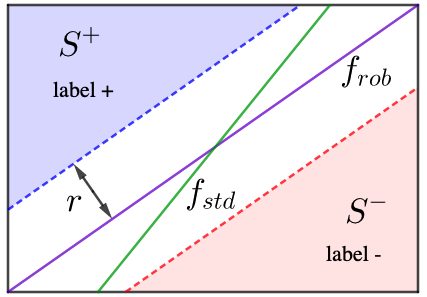
\includegraphics[scale=0.55]{small_margin_robust}
\vspace{.3in}
\caption{An example of a linearly $r$-separated distribution, with positively and negatively labeled examples in $S^+$ and $S^-$ respectively. The optimally robust classifier, $f_{rob}$ is shown in purple, while the (not necessarily unique) optimally accurate classifier, $f_{std}$, is shown in green.}
\label{fig:small_margin_robust}
\end{figure}

\paragraph{General Hypothesis Classes:} We now briefly consider how to extend our methods to other hypothesis classes. For any hypothesis class $\H$ and distribution $\D$ let $$\H_{\D, \alpha} = \{h: h \in \H,\L(h, \D) \leq \alpha\}$$ and let $$\H_{\D, \alpha}^r = \{h: h \in \H,\L_r(h, \D) \leq \alpha\}.$$ $\H_{\D, \alpha}$ can be thought of as the set of accurate classifiers while $\H_{\D, \alpha}^r$ can be thought of as the set of astute classifiers. By their definitions, it is clear that $\H_{\D, \alpha}^r \subseteq \H_{\D, \alpha}$. However, in the case when $\H$ is the set of linear classifiers, we see that for small $\alpha$, $\H_{\D, \alpha}^r$ is a much ``smaller" set than $\H_{\D, \alpha}$. By exploiting the geometric structure inherent to $\H$, we can much more efficiently search for some $h \in \H_{\D, \alpha}$ than we can in $\H_{\D, \alpha}^r$. This dynamic is the crux of our lower bound: as we essentially show that there are far more critical points (i.e. points near the decision boundary) that we must see for learning $\H_{\D, \alpha}^r$ that aren't required for $\H_{\D, \alpha}$. 

Thus, for our methods to extend to an arbitrary hypothesis class, we would require a similar dynamic. We need two properties to hold: (1) $\H_{\D, \alpha}^r$ must be a very strict subset of $\H_{\D, \alpha}$ for sufficiently small alpha. (2) We must have some kind of exploitable geometric structure about $\H$ which allows us to exploit this gap. For the case of linear classifiers, this was the $\ell_2$ measured aspect ratio, $\gamma(\D)$. 

\paragraph{Kernel Classifiers: } A natural choice of a more general hypothesis class would be Kernel Classifiers, which are linear classifiers that operate in an embedded space, $H$. The main difficulty in expanding our lower bound to this more general setting comes from the behavior near the margin: the effects of the robustness radius in the embedded space are considerably less behaved than they are in the standard linear case. Nevertheless, we leave this as an important avenue for future work.

%\begin{algorithm}[H]
%   \caption{Adversarial-Perceptron}
%   \label{alg:upper_bound}
%\begin{algorithmic}[1]
%    \STATE \textbf{Input}:  $S = \{(x_1, y_1), \dots, (x_n, y_n)\} \sim \D^n,$
%    \STATE $w \leftarrow 0$ 
%    \FOR{$i = 1 \dots n$}
%    	\STATE $z = \argmin_{||z - x_i||_p \leq r}  y_i\langle w, z \rangle$ \COMMENT{\rbb{finds adv. ex.}}
%        \IF{$\langle w, y_iz \rangle \leq 0$ \COMMENT{\rbb{checks label}}}
%            \STATE $w \leftarrow w + y_iz$ \COMMENT{\rbb{perceptron update}}
%        \ENDIF           
%    \ENDFOR
%    \STATE return $f_{w, 0}$
%\end{algorithmic}
%\end{algorithm}

\begin{algorithm}[H]
    \SetAlgoLined
    {\bfseries Input:} $S = \{(x_1, y_1), \dots, (x_n, y_n)\} \sim \D^n,$\;
    
    $w \leftarrow 0$ \;
    
    \For{$i = 1 \dots n$}{
    	$z = \argmin_{||z - x_i||_p \leq r}  y_i\langle w, z \rangle$ {\color{red} finds adversarial example}\;
    	
    	\If{$\langle w, y_iz \rangle \leq 0$ {\color{red} checks label}}{
    	
	     	 $w \leftarrow w + y_iz$ {\color{red} perceptron update}\;  	
	     	 
    	}
    }
    
    {\bfseries Return:} $f_{w, 0}$\;
    

\caption{Adversarial-Perceptron}\label{alg:upper_bound}
\end{algorithm}

In the previous section, we showed that for any algorithm, there is some distribution $\D \in \F_{r, \rho}$ that is difficult (i.e. requires high sample complexity) to learn robustly. A natural follow-up question is: what about distributions for which the margin, $\gamma$ is very large compared to $r$. 

Observe that in Figure \ref{fig:small_margin_robust} the robustness radius $r$ is very close to the margin. In particular, we can find adversarial examples from $S^+$ and $S^-$ that are very close to the decision boundary $f_{rob}$. By contrast, if $\gamma >> r$, then this no longer holds which suggests that better robust sample complexities might be possible.

In this section, we will describe a subset of $\F_{r, \rho}$ that can be learned with expected loss $O(\frac{1}{n})$, thus matching the standard sample complexity up to a constant factor. To do so, we will introduce a novel concept: the \textit{robust margin}. The basic intuition is that distributions for which the margin greatly exceeds the robustness radius are precisely distributions with a large robust margin. We use the following notation.

Observe that if $\D$ is a linearly $r$-separated distribution, then $\D$ must also be linearly separable. As earlier, let $S^+, S^- \subset \R^d$ denote the positively and negatively labeled examples from $\D$. We now define \begin{equation}\label{eqn:s_plus_s_minus} S_r^+ = \cup_{s \in S^+} B_p(s, r)\text{ and }S_r^{-} = \cup_{s \in S^-} B_p(s,r).\end{equation} It follows that the decision boundary of any linear classifier with perfect robustness over $\D$ must separate $S_r^+$ and $S_r^-$. We now define the robust margin as a measurement of this separation.

\begin{defn}\label{def:robust_margin}
Let $\D$ be a linearly $r$-separable distribution over $\R^d \times \{\pm 1\}$. Let $S_r^+$ and $S_r^-$ be as above. Then $\D$ has \textbf{robust margin} $\gamma_r$ if $\gamma_r$ is the largest real number such that there exists a linear classifier $f_{w,b}$ with the following properties: 

1. $f_{w,b}$ has perfect astuteness. That is, $\L_r(f_{w,b}, \D) = 0$. 

2. Let $H_{w,b} = \{x: \langle x, w \rangle = b\}$ denote the decision boundary of $f_{w,b}$. Then for all $x \in (S_r^+ \cup S_r^-)$, $x$ has $\ell_2$ distance at least $\gamma$ from $H_{w,b}$. That is, $$\inf_{x \in S_r^+ \cup S_r^-} \inf_{z \in H_{w,b}} ||x - z||_2 \geq \gamma.$$ We let $\gamma_r(\D)$ denote the margin of $\D$, and say that such a distribution is $r, \gamma_r$-separated. 
\end{defn}

It is crucial to note that although adversarial perturbations are measured in $\ell_p$, the robust margin is measured in $\ell_2$. This is because while the metric $\ell_p$ plays a role in constructing $B(x,r)$, it can be completely disregarded once the sets $S_r^+$ and $S_r^-$ are considered, as any hyperplane separating $S_r^+$ and $S_r^-$ will have perfect robustness.  

We now define the robust aspect ratio, which is the robust analog of standard aspect ratio.

\begin{defn}
Let $\D$ be a distribution over $\R^d \times \{\pm 1\}$. Then the \textbf{robust aspect ratio} of $\D$, $\rho_r(\D)$ is defined as $$\rho_r(\D) = \frac{diam_2(S_r^+ \cup S_r^-)}{\gamma_r(\D)},$$ where as before, $diam_2(S_r^+ \cup S_r^-)$ denotes its diameter in the $\ell_2$ norm.
\end{defn}

We will now show that just as the aspect ratio, $\rho(\D)$, characterized the sample complexity for standard classification, the robust aspect ratio, $\rho_r(\D)$ will characterize the sample complexity for robust learning. To do so, we present a perceptron-inspired algorithm (Algorithm \ref{alg:upper_bound}) for learning a robust classifier on $r$-separated data with robust aspect ratio $\rho_r$. 

The basic idea behind Algorithm \ref{alg:upper_bound} is to combine the standard perceptron algorithm with adversarial training. In particular, we iterate through the training set and do the following on each point (refer to Algorithm \ref{alg:upper_bound} for precise details). 

1. Find an adversarial example $(z, y_i)$ by attacking our classifier, $f_{w, 0}$, at $(x_i, y_i)$ (line 4). This is a straightforward convex optimization problem for linear classifiers.

2. If $f_{w,0}(z) \neq y_i$, we update our weight vector with $(z, y_i)$ by using the standard perceptron update (lines 5-6).

We have the following upper bound on the expected robust loss of our algorithm.

\begin{thm}\label{thm:upper_bound}
Let $\D$ be a distribution with robust aspect ratio $\rho_r(\D)$. Then for any $n > 0$, we have $$\E_{S \sim \D^n} [\L_r(A_S, \D)] \leq O(\frac{\rho_r(\D)^2}{n}),$$ where $A_S$ denotes the classifier learned by Algorithm \ref{alg:upper_bound} from training data $S$. 
\end{thm}

Observe that this expected loss is still larger than the expected standard loss in  Theorem \ref{thm:standard} as $\rho_r(\D) > \rho(\D)$ for any $\D$. We also note that this result is not contradictory with our lower bound; there exist distributions $\D \in \F_{r, \rho}$ such that $\gamma_r(\D) = 0$, and these are precisely the distributions for which our lower bounds hold.

\subsection{Generalization to Kernel Classifiers}

Algorithm \ref{alg:upper_bound} can be thought of as the robust analog to the perceptron algorithm. We now generalize this algorithm to obtain a robust variant of the \textit{kernel perceptron algorithm}. We first briefly review kernel classifiers. A detailed explanation of our generalized algorithm along with requisite background material can be found in Appendix \ref{sec:kernel_appendix}

\begin{defn}\label{defn:kernel}
Let $K: \R^d \times \R^d \to \R$ be a kernel similarity function, $T = \{(x_1, y_1), \dots, (x_m, y_m)\} \subset \R^d \times \{\pm 1\}$ be a set of labeled points, and $\alpha \in \R^m$ be a vector of $m$ real numbers. Then the \textbf{kernel classifier} with similarity function $K$, parameters $T, \alpha$, and denoted by $f_{T, K}^\alpha$ is defined as $$f_{T, \alpha}^K(x) = \begin{cases} +1 &  \sum_1^m \alpha_iy_iK(x_i, x) \geq 0\\ -1 &  \sum_1^m \alpha_iy_iK(x_i, x) < 0  \end{cases}.$$
\end{defn}

Conceptually, kernel classifiers are linear classifiers operating in embedded space. With each kernel similarity function $K$, there is a map $\phi: \R^d \to H$ (where $H$ is some Hilbert space) such that $K(x, x') = \langle \phi(x), \phi(x') \rangle$. Thus we can think of kernel classifiers as having a linear decision boundary in $H$. 

We now present an analog of Algorithm \ref{alg:upper_bound} that we call the Adversarial Kernel-Perceptron. The essence of this algorithm has not changed. For each $(x_t, y_t)$ in our training set, we do the following.

1. Find an adversarial example $(z, y_i)$ by attacking our classifier, $f_{T, \alpha}^K$, at $(x_i, y_i)$ (line 4). 

2. If $f_{T, \alpha}^K(z) \neq y_i$, we update our weight vector with $(z, y_i)$ by appending $(z, y_i)$ to $T$ lines (5-6). This corresponds to a kernel-perceptron update that uses $(z, y_i)$ instead of $(x_i, y_i)$.

\begin{algorithm}[H]

\textbf{Input}:  $S = \{(x_1, y_1), \dots, (x_n, y_n)\} \sim \D^n,$ Similarity function, $K$

$T \leftarrow \emptyset$, $\alpha \leftarrow 0$

\For{$i = 1 \dots n$}{
    	$z = \argmin_{||z - x||_p \leq r}  y_if_{T, \alpha}^K(z)$ {\color{red}finds adv. ex.}
    	
        \If{$f_{T, \alpha}^k(z) \leq 0$ {\color{red} checks label}}{
        
            $T = T \cup \{(z, y_i)\}$ {\color{red} kern. percep. update}
            
            $\alpha = (1, \dots, 1)_{|T|}$
            
         }
}
        
Return $f_{T, \alpha}^K$
   \caption{Adversarial-Kernel-Perceptron}
   \label{alg:upper_bound_kernel}
\end{algorithm}

One challenging aspect of this algorithm is minimizing $f_{T, \alpha}^k(z)$. For linear classifiers, this has a closed form solution that utilizes the dual norm. For arbitrary Kernel classifiers, this is a somewhat more challenging problem. However, we note that this can be solved using standard optimization techniques, and in some cases (when $K$ is particularly simple), it can be solved with basic gradient descent.

Finally, we show that this Algorithm has similar performance to the linear case. Instead of using the robust aspect ratio, $\rho_r(\D)$, to bound the performance, we will require the \textbf{robust $K$-aspect ratio}, which is the kernel analog of this quantity. It can be thought of as the robust aspect ratio in the embedded space $H$. Details about this quantity (along with the proof of the theorem) can be found in Appendix \ref{sec:kernel_appendix}.

\begin{thm}\label{thm:upper_bound_kernel}
Let $\D$ be a distribution with robust $K$-aspect ratio $\rho_r^K(\D)$. Then for any $n > 0$, we have $$\E_{S \sim \D^n} [\L_r(A_S, \D)] \leq O(\frac{\rho_r^K(\D)^2}{n}),$$ where $A_S$ denotes the classifier learned by Algorithm \ref{alg:upper_bound_kernel} from training data $S$. 
\end{thm}

This result indicates that for small values of $\rho_r^k(\D)$, we can achieve a very good robust sample complexity for kernel classifiers. However, as the size of the perturbations approach this margin, this quantity goes to infinity. This phenomenon mirrors the linearly separable case, and suggests that a similar overall dynamic holds for kernel classification. We leave finding a full generalization (including our lower bound) for a direction in future work.






%\input{chapters/chapter1/macros}
%\input{chapters/chapter1/introduction}
%\input{chapters/chapter1/related}
%\input{chapters/chapter1/definition}
%\input{chapters/chapter1/quantifying}
%\input{chapters/chapter1/visualizing}
%\input{chapters/chapter1/mitigation}